\documentclass[journal,10pt]{IEEEtran}
% \documentclass[11pt,draftcls,onecolumn]{IEEEtran}
% \documentclass[a4paper,10pt]{article}

\usepackage{amsmath}
\usepackage{amsfonts}
%\usepackage{IEEEtrantools}
\usepackage{algorithm}
\usepackage{algorithmic}
% \usepackage{graphicx}
\usepackage{hyperref}
\usepackage[caption=false]{subfig}
\usepackage{cite}

\usepackage{tikz}
\usepackage{pgfplots}
\usepgfplotslibrary{groupplots}
 \usetikzlibrary{plotmarks}
 \pgfplotsset{compat=newest}
 \pgfplotsset{plot coordinates/math parser=false}
 \usepgfplotslibrary{external}
 \tikzexternalize[prefix=tikz/]

% Mathematical basics
\newcommand{\half}{\frac{1}{2}}
\newcommand{\zmat}[1][]{0_{#1}}
\newcommand{\idmat}[1][]{I_{#1}}
\newcommand{\reals}{\mathbb{R}}
\newcommand{\naturals}{\mathbb{N}^{+}}
\newcommand{\bigo}{\mathcal{O}}

% Functions
\newcommand{\gammafun}[1][]{\Gamma_{#1}}

% Operations
\DeclareMathOperator{\trace}{Tr}
\DeclareMathOperator{\diag}{Diag}
\DeclareMathOperator{\vectorise}{Vec}
\DeclareMathOperator{\rank}{Rank}
\DeclareMathOperator{\sign}{Sign}
\newcommand{\inv}{^{-1}}
\newcommand{\pinv}{^{+}}
\newcommand{\tr}{^{T}}
\newcommand{\invtr}{^{-T}}
\newcommand{\msqrt}{^{\half}}
\newcommand{\determ}[1]{\left|#1\right|}
\newcommand{\volel}[1]{\left(#1\right)}
\newcommand{\hadprod}{\circ}
\newcommand{\kronprod}{\otimes}
\newcommand{\jac}{J}

% Distribution families ...
\newcommand{\normaldist}[2]{\mathcal{N}\left(#1,#2\right)}
\newcommand{\wishartdist}[2]{\mathcal{W}\left(#1,#2\right)}
\newcommand{\iwishartdist}[2]{\mathcal{IW}\left(#1,#2\right)}
\newcommand{\matrixnormaldist}[3]{\mathcal{MN}\left(#1,#2,#3\right)}

% ... and their ``densities''
\newcommand{\normalden}[3]{\mathcal{N}\left(#1\middle|#2,#3\right)}
\newcommand{\matrixnormalden}[4]{\mathcal{MN}\left(#1\middle|#2,#3,#4\right)}
\newcommand{\wishartden}[3]{\mathcal{W}\left(#1\middle|#2,#3\right)}
\newcommand{\iwishartden}[3]{\mathcal{IW}\left(#1\middle|#2,#3\right)}
\newcommand{\gammaden}[3]{\mathcal{G}\left(#1\middle|#2,#3\right)}
\newcommand{\igammaden}[3]{\mathcal{IG}\left(#1\middle|#2,#3\right)}
\newcommand{\bernoulliden}[2]{\mathcal{BER}\left(#1\middle|#2\right)}
\newcommand{\diracden}[2]{\delta_{#2}\left(#1\right)}

% Time indexes
\newcommand{\ti}{t}
\newcommand{\timax}{T}

% Dimensions
\newcommand{\lsd}{d_x}
\newcommand{\obd}{d_y}
\newcommand{\rk}{r}

% Densities
\newcommand{\den}{p}
\newcommand{\postden}{\pi}
\newcommand{\ppslden}[1]{q_{#1}}

% State space model variables
\newcommand{\ls}[1]{x_{#1}}
\newcommand{\ob}[1]{y_{#1}}
\newcommand{\tn}[1]{\epsilon^{x}_{#1}}
\newcommand{\on}[1]{\epsilon^{y}_{#1}}
\newcommand{\LS}[1]{X_{#1}}

% State space model parameters                          % Linear Gaussian ...
\newcommand{\lgtm}[1][]{F_{#1}}                         % transition matrix
\newcommand{\lgtv}[1][]{Q_{#1}}                         % transition variance
\newcommand{\lgom}{H}                                   % observation matrix
\newcommand{\lgov}{R}                                   % observation variance
\newcommand{\lgdm}{G}                                   % disturbance matrix

% Factorisations for the covariance matrix
\newcommand{\tvval}{\Lambda}
\newcommand{\tvvec}{V}
\newcommand{\tvvecorth}{V_{\perp}}
\newcommand{\tvfull}{D}
\newcommand{\tvrot}{U}
\newcommand{\tvrotorth}{U_{\perp}}
\newcommand{\eval}[1]{\lambda_{#1}}
\newcommand{\evec}[1]{v_{#1}}
\newcommand{\evecset}[1]{\mathcal{V}_{#1}}
\newcommand{\tvrow}{U_R}
\newcommand{\tvcross}{U_C}
\newcommand{\tvsign}{E}
\newcommand{\tvsigndiag}{\tilde{E}}

% Givens rotations
\newcommand{\givrot}[1]{\gamma_{#1}}
\newcommand{\givmat}[3]{\Gamma_{#1,#2}(#3)}

% Projections
\newcommand{\lgtmrot}{F_U}
\newcommand{\lgtmorth}{F_{\perp}}

% Hyperparameters
\newcommand{\priordof}{\nu_0}
\newcommand{\priorscalematrix}{\Psi_0}
\newcommand{\priorscalematrixrank}[1]{\Psi_{0}^{[#1]}}
\newcommand{\priorscalematrixbase}{\Psi_0^{[1]}}
\newcommand{\priorcolumnvariance}{\Omega_0}
\newcommand{\priormeanmatrix}{M_0}
\newcommand{\priorextratpval}{\Lambda_{\perp}}
\newcommand{\priortypval}{\alpha}
\newcommand{\priorrankweight}[1]{w_{#1}}
\newcommand{\postdof}{\nu}
\newcommand{\postscalematrix}{\Psi}
\newcommand{\postcolumnvariance}{\Omega}
\newcommand{\postmeanmatrix}{M}
\newcommand{\suffstats}[1]{S_{#1}}

% Transition precision MH
\newcommand{\mhrot}{\Xi}
\newcommand{\mhrotppsl}{\varsigma}

% Transition matrix MH
\newcommand{\padding}{\delta}
\newcommand{\paddedlgtv}{\widetilde{\lgtv}}

% Markov Chains
\newcommand{\mcold}{^*}
\newcommand{\mcnew}{^{\prime}}
\newcommand{\mhap}{\alpha}
\newcommand{\mhar}{\beta}
\newcommand{\jacob}{J}

% Generic variables
\newcommand{\psd}{\Upsilon}






%%%%%%% OLD ONES - DELETE THES!! %%%%%%%%%

% State space model parameters
\newcommand{\lgtp}[1][]{\Upsilon_{#1}}

% Degenerate state space model parameters
\newcommand{\lgtnm}{G}
\newcommand{\tnmo}{V}
\newcommand{\tnmd}{\Lambda}
\newcommand{\tnmf}{D}
\newcommand{\tnmev}[1]{\lambda_{#1}}
\newcommand{\tnmevec}[1]{v_{#1}}
\newcommand{\tnmofull}{\widetilde{V}}
\newcommand{\tnmocross}{U_{C}}
\newcommand{\tnmocrossred}{U}%{\tilde{U}_{C}}
\newcommand{\tnmocrossrem}{\widetilde{U}}%{\breve{U}_{C}}
\newcommand{\tnmorow}{U_{R}}
\newcommand{\tnmonullred}{\widetilde{U}_{N}}
\newcommand{\tnmorowred}{\widetilde{U}_{R}}
\newcommand{\tnmonull}{U_{N}}
\newcommand{\tnmosign}{E}
\newcommand{\tnmosignred}{\widetilde{E}}


\newcommand{\meta}[1]{{\color{red}\em #1}}

%opening
\title{Bayesian Learning of Degenerate Linear~Gaussian~State~Space~Models using~Markov~Chain~Monte~Carlo}
\author{Pete Bunch$^*$, James Murphy and Simon Godsill
  \thanks{Department of Engineering, University of Cambridge, Cambridge, UK.}
  \thanks{Email: $\{$pb404,jm362,sjg30$\}$@cam.ac.uk}%
}

\begin{document}

\maketitle



\begin{abstract}
Linear Gaussian state space models are ubiquitous in signal processing, and an important procedure is that of estimating system parameters from observed data. Rather than making a single point estimate, it is often desirable to conduct Bayesian learning, in which the entire posterior distribution of the unknown parameters is sought. This can be achieved using Markov chain Monte Carlo. On some occasions it is possible deduce the form of the unknown system matrices in terms of a small number of scalar parameters, by considering the underlying physical processes involved. Here we study the case where this is not possible, and the entire matrices must be treated as unknowns. An efficient Gibbs sampling algorithm exists for the basic formulation of linear model. We extend this to the more challenging situation where the transition model is degenerate. Appropriate Markov kernels are devised and demonstrated with simulations.
\end{abstract}



\section{Introduction}

State space models are frequently used to describe time-varying systems, and Linear Gaussian models in particular are ubiquitous throughout signal processing. The physical phenomena modelled within this framework include the kinematics of moving targets \cite{Bar-Shalom2002}, audio signals \cite{Godsill1998}, genetic networks \cite{Beal2005}, and many others. The popularity of linear Gaussian state space models stems in part from their analytic tractability. Inference tasks can be performed in closed form using algorithms such as the Kalman filter \cite{Kalman1960} and Rauch-Tung-Striebel (RTS) smoother \cite{Rauch1965}.

A linear Gaussian state space model is specified by a number of system matrices which govern the latent state and observation processes. An important consideration is how to learn these fixed matrices from observed data. The parametric approach to this problem is to deduce the form of the system matrices in terms of a small number of scalar parameters by considering the physical mechanisms underlying the system, and then attempt to learn these. (See e.g. \cite{Kantas2009,Andrieu2010}.) However, in many systems there may not be an obvious parametric form, and it may be better to treat each system matrix in its entirety as an unknown variable to be learned. This type of non-parametric learning for linear Gaussian state space models is the focus of this paper. There is a large body of research on this topic, which has generally concentrated on point estimate methods. These include subspace identification approaches \cite{VanOverschee1991,Viberg1995}, and maximum likelihood estimates using either gradient-based algorithms (see e.g. \cite{Cappe2005,Sarkka2013}) or Expectation-Maximisation (EM) \cite{Shumway1982,Digalakis1993,Ghahramani1996,Gibson2005,Li2009}.

More recently, Bayesian approaches have been developed for non-parametric learning of linear Gaussian state space models, in which full posterior distributions for the system parameters are calculated. Since this is not possible analytically (see discussion in \cite{Beal2003}), approximations must be employed. One possibility is to take a variational approach, approximating the full joint posterior distribution as a product of independent marginals \cite{Ghahramani2001,Beal2003,Barber2007}. Alternatively, the true joint posterior can be targeted using Markov chain Monte Carlo (MCMC). This has the advantage of providing consistent estimates not only of the system matrices but also of any function of these quantities (e.g. phase margins, system poles). The price we pay is in computation; it is necessary to allow the Markov chains to run until convergence in order to form good estimates. Generic Metropolis-Hastings strategies such as those adopted in \cite{Ninness2010} are liable to mix very slowly and exact too great a computational demand. However, if conjugate priors are assumed for the various system matrices, then a Gibbs sampler may be implemented which attains substantially improved efficiency and requires almost no algorithm tuning \cite{Wills2012}.

The Gibbs sampler approach developed in \cite{Wills2012} is effective on the basic flavour of linear Gaussian state space models. However, it is not able to handle the case in which the transition model is degenerate, i.e. when the transition covariance matrix is not full rank. In this paper we extend the MCMC learning framework to encompass this scenario. This is achieved by appropriate factorisations of the covariance matrix which allow us still to exploit the fast-mixing Gibbs kernel. Furthermore, reversible jump construction \cite{Green1995,Green2009} is introduced which enables the sampler to learn the rank of the transition covariance matrix.

%and parameterising the attainable subspace using a set of Givens rotations \cite{Anderson1987,Shalit2014,Yang1994,Cao2011,Cron2014}.

The paper is structured as follows. In section~\ref{sec:linear_gaussian_models} we review the Gibbs sampler for basic linear Gaussian state space systems, focusing on the transition model. In section~\ref{sec:degenerate_transition_models} we describe modifications for degenerate transitions, and in section~\ref{sec:rank_learning} we show how the rank of the transition covariance may be learned. Simulations on a toy model, and a motion capture application are presented in section~\ref{sec:simulations}.


% Citations which might be useful
% Linear systems with stability constraints: \cite{Boots2008}
% Givens rotations: \cite{Yang1994,Cao2011,Cron2014} (for covariance) \cite{Anderson1987,Shalit2014} (for generic orthogonal matrixes)



\section{Basic Linear Gaussian Models} \label{sec:linear_gaussian_models}
State space models are used to represent time-varying systems, and consist of a latent state process $\{\ls{\ti}\}_{\ti=1:\timax}$ and a related observation process $\{\ob{\ti}\}_{\ti=1:\timax}$. The challenge is to infer the sequence of unknown latent states, and learn parameters of the model, from the sequence of known observations. It is usually assumed that the state process is Markovian (i.e. $\ls{\ti}|\ls{\ti-1}$ is independent of $\ls{1:\ti-2}$) and that each observation depends only on the current state (i.e. $\ob{\ti}|\ls{\ti}$ is independent of $\ls{1:\ti-1}$ and $\ls{\ti+1:\timax}$).

A basic linear state space model therefore obeys the following recursive system equations,
%
\begin{IEEEeqnarray}{rCl}
 \ls{\ti} & = & \lgtm \ls{\ti-1} + \tn{\ti} \\
 \ob{\ti} & = & \lgom \ls{\ti}   + \on{\ti}       ,
\end{IEEEeqnarray}
%
where $\ls{\ti} \in \reals^{\lsd}$ and $\ob{\ti} \in \reals^{\obd}$. In addition, we assume the state disturbance and observation noise variables have a Gaussian distribution,
%
\begin{IEEEeqnarray}{rCl}
 \tn{\ti} & \sim & \normalden{\tn{\ti}}{0}{\lgtv} \\
 \on{\ti} & \sim & \normalden{\on{\ti}}{0}{\lgov}     ,
\end{IEEEeqnarray}
%
where $\lgtv$ and $\lgov$ are positive definite covariance matrices. This model can be written equivalently in terms of transition and observation densities,
%
\begin{IEEEeqnarray}{rCl}
 \den(\ls{\ti}|\ls{\ti-1},\lgtm,\lgtv) & = & \normalden{\ls{\ti}}{\lgtm\ls{\ti-1}}{\lgtv} \\
 \den(\ob{\ti}|\ls{\ti},\lgom,\lgov)   & = & \normalden{\ob{\ti}}{\lgom\ls{\ti}}{\lgov}      .
\end{IEEEeqnarray}
%
The initial state $\ls{1}$ may be known or may be assigned a Gaussian prior.

The system is parameterised by the four matrices $\left\{\lgtm, \lgom, \lgtv, \lgov\right\}$. In this paper we focus on learning the transition model, i.e. $\lgtm$ and $\lgtv$, and treat $\lgom$ and $\lgov$ as fixed and known throughout. Conditional on these matrices, state inference may be carried out analytically. Posterior filtering and smoothing densities may be calculated using the Kalman filter \cite{Kalman1960} and Rauch-Tung-Striebel (RTS) smoother \cite{Rauch1965}. Furthermore, the Kalman filter may also be used to evaluate the marginal likelihood $\den(\ob{1:\timax}|\lgtm, \lgtv)$, and it is possible to draw posterior samples from the state posterior $\den(\ls{1:\timax}|\ob{1:\timax}, \lgtm, \lgtv)$ using the forward-filtering-backward-sampling method \cite{Chib1996}. The purpose of a learning algorithm is estimate unknown values of $\left\{\lgtm, \lgtv\right\}$ from a sequence of observations. Within the Bayesian framework this means calculating or approximating the posterior distribution $\den(\lgtm, \lgtv|\ob{1:\timax})$, which we can achieve using MCMC. 

In order to conduct Bayesian learning, we first need to define prior distributions for the unknown system matrices $\lgtm$ and $\lgtv$. Although these should be selected to reflect prior belief about the system in question, there is substantial benefit in using conjugate priors, as these enable us to use Gibbs sampling moves. Typically, we will not have strong prior beliefs about the parameters, so it is reasonable to use an uninformative conjugate prior. However, if we do have prior knowledge to take into account which means that a conjugate prior is not appropriate, then we can treat each Gibbs move as a proposal in a Metropolis-Hastings scheme and use an accept/reject stage to account for the difference between the true prior and the conjugate prior used for the sampling \cite{Wills2012}.



\subsection{System Matrix Priors}

The conjugate prior for $\lgtm, \lgtv$ is a matrix normal--inverse Wishart distribution \cite{Wills2012},
%
\begin{align}
 \lgtv &\sim \iwishartdist{\priordof}{\priorscalematrix} \\
 \lgtm | \lgtv &\sim \matrixnormaldist{\priormeanmatrix}{\lgtv}{\priorcolumnvariance}     ,
\end{align}
%
with the following density function,
%
\begin{equation}
 \den(\lgtm, \lgtv) =  \den(\lgtm | \lgtv) \den(\lgtv)
\end{equation}
%
\begin{IEEEeqnarray}{rCl}
\den(\lgtv) &=& \frac{ \determ{\priorscalematrix}^{\frac{\priordof}{2}} }{ 2^{\frac{\priordof}{2}} \gammafun\left(\frac{\priordof}{2}\right) } \determ{\lgtv}^{-\frac{\priordof+\lsd+1}{2}} \exp\left( -\half \trace\left[\lgtv\inv\priorscalematrix\right] \right) \nonumber \\
\\
\den(\lgtm | \lgtv) &=& \determ{2 \pi \lgtv}^{-\half} \determ{2 \pi \priorcolumnvariance}^{-\half} \nonumber \\
& & \times \exp\left(-\half \trace\left[ \lgtv\inv (\lgtm-\priormeanmatrix) \priorcolumnvariance\inv (\lgtm-\priormeanmatrix)\tr \right] \right) \nonumber \\
\end{IEEEeqnarray}
%
$\priordof\in\reals, \priordof>\lsd-1$. $\priorscalematrix$ and $\priorcolumnvariance$ are $\lsd\times\lsd$ positive definite matrices. $\priormeanmatrix \in \reals^{\lsd\times\lsd}$.



\subsection{Gibbs Sampling for Basic Linear Gaussian Models}

Our principal interest is to learn the system matrices $\lgtm$ and $\lgtv$ from a sequence of observations $\ob{1:\timax}$. The appropriate posterior distribution is not amenable to efficient MCMC sampling, so instead we introduce the latent state sequence $\ls{1:\timax}$ as a nuisance variable and target the joint posterior,
%
\begin{IEEEeqnarray}{rCl}
 \postden(\lgtm, \lgtv, \ls{1:\timax}) & = & \den(\lgtm, \lgtv, \ls{1:\timax} | \ob{1:\timax}) \\
 & \propto & \den(\ob{1:\timax}|\ls{1:\timax}) \den(\ls{1:\timax}|\lgtm,\lgtv) \den(\lgtm|\lgtv) \den(\lgtv) \nonumber      .
\end{IEEEeqnarray}

An appropriate Gibbs sampler can be constructed by sampling alternately from the following conditional posterior distributions,
%
\begin{IEEEeqnarray}{l}
 \postden(\ls{1:\timax}|\lgtm, \lgtv) \nonumber \\
 \postden(\lgtm, \lgtv| \ls{1:\timax}) \nonumber      .
\end{IEEEeqnarray}
%
The distribution of the sampled values will then converge to the target posterior distribution \cite{Roberts1994}. The state conditional $\postden(\ls{1:\timax}|\lgtm, \lgtv)$ can be sampled using the forward-filtering-backward-sampling algorithm \cite{Chib1996,Wills2012}, which works by first running a Kalman filter forwards through the data, then running backwards in time sampling each state conditional on those in the future. The parameter conditional may also be sampled directly. This depends on the state sequence probability,
%
\begin{IEEEeqnarray}{rCl}
 \IEEEeqnarraymulticol{3}{l}{ \den(\ls{1:\timax}|\lgtm,\lgtv) \propto \prod_{\ti=2}^{\timax} \den(\ls{\ti}|\ls{\ti-1},\lgtm,\lgtv) } \\
 & \propto & \determ{\lgtv}^{-\frac{\timax-1}{2}} \exp\left( -\half \sum_{\ti=2}^{\timax} (\ls{\ti}-\lgtm\ls{\ti-1})\tr \lgtv\inv (\ls{\ti}-\lgtm\ls{\ti-1}) \right) \nonumber      .
\end{IEEEeqnarray} 

It is straightforward to show that the required conditional distribution is also a matrix normal--inverse Wishart distribution \cite{Wills2012},
%
\begin{IEEEeqnarray}{rCl}
 \lgtv | \ls{1:\timax} &\sim& \iwishartdist{\postdof}{\postscalematrix} \\
 \lgtm | \lgtv, \ls{1:\timax} &\sim& \matrixnormaldist{\postmeanmatrix}{\lgtv}{\postcolumnvariance}     ,
\end{IEEEeqnarray}
%
with the following updated hyperparameters,
%
\begin{align}
 \postcolumnvariance\inv                 &= \priorcolumnvariance\inv + \suffstats{1} \nonumber \\
 \postmeanmatrix \postcolumnvariance\inv &= \priormeanmatrix \priorcolumnvariance\inv + \suffstats{2} \nonumber \\
 \postdof                                &= \priordof + \suffstats{0} \nonumber \\
 \postscalematrix                        &= \priorscalematrix + \suffstats{3} + \priormeanmatrix \priorcolumnvariance\inv \priormeanmatrix\tr - \postmeanmatrix \postcolumnvariance\inv \postmeanmatrix\tr    ,
\end{align}
%
in which the following sufficient statistics are used,
%
\begin{IEEEeqnarray}{rClCrCl}
 \suffstats{0} &=& \timax - 1 & \qquad & \suffstats{1} &=& \sum_{t=2}^{\timax} \ls{\ti-1}\ls{\ti-1}\tr \nonumber \\
 \suffstats{2} &=& \sum_{t=2}^{\timax} \ls{\ti}\ls{\ti-1}\tr & \qquad & \suffstats{3} &=& \sum_{t=2}^{\timax} \ls{\ti}\ls{\ti}\tr      .
\end{IEEEeqnarray}

Both matrix normal and inverse Wishart distributions may be sampled using standard methods. Hence we have all the components necessary to implement a Gibbs sampler for this model.



\section{Degenerate Transition Models} \label{sec:degenerate_transition_models}

A commonly encountered variation on the basic linear Gaussian state space model is as follows,
%
\begin{IEEEeqnarray}{rCl}
 \ls{\ti} & = & \lgtm \ls{\ti-1} + \lgdm \tn{\ti} \label{eq:degenerate_transition} \\
 \tn{\ti} & \sim & \normalden{\tn{\ti}}{0}{\idmat}      ,
\end{IEEEeqnarray}
%
in which $\tn{\ti}$ as dimension $\rk$, and $\lgdm$ is $\lsd\times\rk$. This is almost equivalent to the previous, with $\lgtv=\lgdm\lgdm\tr$. However, whereas before $\lgtv$ was required to be positive definite, this is no longer the case. When this occurs, the conventional transition density $\den(\ls{\ti}|\ls{\ti-1},\lgtm,\lgdm)$ is not defined, and the sampling operations underlying our Gibbs sampler are no longer valid. Degenerate models such as these arise in tracking applications (see \cite{Maskell2004} for a discussion of this phenomenon); when non-Markovian models, such as autoregressive process, are converted to state space form; and when it is natural to parameterise a system with more latent states than there are degrees of freedom (see section~\ref{sec:mocap}). In this section, we introduce a parameterisation for such degenerate transition models which can uniquely represent any such system, and show how MCMC moves may be implemented for learning. Here we treat $\rk$ as fixed and known; in the following section mechanisms will be introduced to learn this too.

The matrix $\lgdm$ is not uniquely identifiable from the state sequence, because the distribution of $\lgdm\tn{\ti}$ is identical to that of $\lgdm \Xi \tn{\ti}$ where $\Xi$ is an arbitrary orthogonal matrix. To avoid this ambiguity, it is better to focus on learning $\lgtv$ as before, and to define $\lgdm$ as some matrix square root of $\lgtv$ (e.g. the Cholesky factor or the principal matrix square root). In this new setting, $\lgtv$ is a positive semi-definite matrix with rank $\rk$.

There are two difficulties with extending the methodology from the basic model to the degenerate case. First, the conjugate matrix normal--inverse Wishart distribution becomes singular. This places an undesirable constraint on the transition matrix which needs to be removed. Second, each transition, $(\ls{\ti}-\lgtm\ls{\ti-1})$, is now constrained to lie in a particular $\rk$-dimensional subspace within the state space; specifically, within the column space of $\lgdm$. This subspace is fixed conditional on any sampled state trajectory $\ls{1:\timax}$ (provided that $\timax>\rk$). This makes standard Gibbs sampling from $\postden(\lgtm, \lgtv|\ls{1:\timax})$ insufficient, since there are values of $\lgtm$ and $\lgtv$ which can never be reached.

There is an obvious way to avoid being constrained to a particular subspace by the sampled state trajectory; simply return to targeting the marginal posterior $\postden(\lgtm, \lgtv|\ob{1:\timax})$ and fall back to using a generic Metropolis-Hastings approach. However, with a complex and high dimensional parameter space, designing efficient proposal distributions for Metropolis-Hastings is difficult. We would prefer to attain the automated, fast-mixing properties displayed by the Gibbs sampler on the full rank model. In this section we show how a Gibbs kernel may still be applied to sample a component of the parameters, with the remainder handled using Metropolis-Hastings.

In formulating an MCMC algorithm for degenerate transition models, we will make use of two factorisations of the transition covariance matrix. First, an eigendecomposition,
%
\begin{IEEEeqnarray}{rCl}
 \lgtv &=& \tvvec \tvval \tvvec\tr     ,
\end{IEEEeqnarray}
%
in which $\tvval$ is a diagonal $\rk\times\rk$ matrix with $\rk = \rank(\lgtv)$, and $\tvvec$ is a $\lsd\times\rk$ matrix of orthonormal columns from the appropriate Stiefel manifold. This is the ``non-singular'' part of the factorisation. In order to resolve ambiguities in this representation, we follow \cite{Muirhead1982} and require that the first element in each column of $\tvvec$ should be positive, and that eigenvalues in $\tvval$ be arranged in decreasing order of magnitude. The transformation from $\lgtv$ to $\{\tvval, \tvvec\}$ is then bijective.

We can also write the ``full'' factorisation by finding a set of $\lsd-\rk$ additional orthonormal vectors and appending them to $\tvvec$, along with matching zeros to $\tvval$, as follows,
%
\begin{IEEEeqnarray}{rCl}
 \lgtv &=& \begin{bmatrix}\tvvec & \tvvecorth \end{bmatrix} \begin{bmatrix}\tvval & \zmat \\ \zmat & \zmat \end{bmatrix} \begin{bmatrix}\tvvec\tr \\ \tvvecorth\tr \end{bmatrix}
\end{IEEEeqnarray}
%
Note that $\tvvecorth$ is not unique. 

A further factorisation will also be useful, which we will refer to as the Givens decomposition (on account of its method of computation). For the rank-$\rk$ positive semi-definite covariance matrix $\lgtp$,
%
\begin{IEEEeqnarray}{rCl}
 \lgtv &=& \tvrot \tvfull \tvrot\tr \label{eq:givens_decomposition} %&=& \begin{bmatrix}\tvrot & \tvrotorth\end{bmatrix} \begin{bmatrix}\tvfull & \zmat \\ \zmat & \zmat\end{bmatrix} \begin{bmatrix}\tvrot\tr \\ \tvrotorth\tr\end{bmatrix}
\end{IEEEeqnarray}
%
where,
%
$\tvfull$ is a $\rk\times\rk$ positive definite matrix and $\tvrot$ is a $\lsd\times\rk$ matrix of orthonormal vectors subject to certain constraints. The transformation from $\lgtv$ to $\{\tvfull, \tvrot\}$ is also bijective. See appendix~\ref{app:givens-factorisation} for details.


\subsection{Degenerate Transition Priors}

The matrix normal--inverse Wishart conjugate prior will need some modifications in order to apply it to degenerate models.

An appropriate prior distribution for the degenerate transition covariance matrix may be defined by setting the degrees of freedom of an inverse Wishart distribution to the desired rank, $\priordof=\rk$. This results in a singular inverse Wishart distribution over the rank-$\rk$ positive semi-definite matrices \cite{Diaz-Garcia2006},
%
\begin{IEEEeqnarray}{rCl}
 \lgtv|\rk &\sim& \iwishartdist{\rk}{\priorscalematrixrank{\rk}}     .
\end{IEEEeqnarray}
%
The density (with respect to the Lesbegue measure on the distinct elements) is,
%
\begin{IEEEeqnarray}{rCl}
 \den(\lgtv|\rk) &=& \frac{ \determ{\priorscalematrixrank{\rk}}^{\frac{\rk}{2}} }{ 2^{\half\rk\lsd} \pi^{\half\rk(\lsd-\rk)} \gammafun[r]\left(\frac{\rk}{2}\right) } \nonumber \\
 & & \qquad \times \determ{\tvval}^{-\half(3\lsd-\rk+1)} \exp\left( -\half \lgtv\pinv \priorscalematrixrank{\rk} \right)    ,
\end{IEEEeqnarray}
%
in which $\lgtv\pinv$ denotes the Moore-Penrose pseudoinverse of $\lgtv$. A prior estimate of $\lgtv$ is $\frac{1}{\rk}\priorscalematrixrank{\rk}$. Thus, in order to maintain consistency between the different ranks, we should set $\priorscalematrixrank{\rk} = \rk \priorscalematrixbase$, where $\priorscalematrixbase$ is an estimate of $\lgtv$.

The matrix normal component of the prior is more problematic. Although the distribution it is still well-defined, the fact that $\lgtv$ is singular means that the space of possible values is restricted to a subspace of $\reals^{\lsd\times\lsd}$, placing an unwanted constraint on our model. (See \cite{Diaz-Garcia2006} for a discussion of the singular matrix normal distribution.)

In order to relax this unwanted constraint, the following non-singular prior distribution may be used,
%
\begin{IEEEeqnarray}{rCl}
 \lgtm|\lgtv &\sim& \matrixnormaldist{\priormeanmatrix}{\lgtv+\tvvecorth\priorextratpval\tvvecorth\tr}{\priorcolumnvariance}
\end{IEEEeqnarray}
%
in which $\priorextratpval$ is a diagonal matrix of positive eigenvalues. The matrix $\lgtv+\tvvecorth\priorextratpval\tvvecorth\tr$ is then guaranteed to be positive definite.

Using this prior, we need a mechanism for choosing $\priorextratpval$. These extra eigenvalues control the rate at which probability decays as the matrix moves away from the subspace defined by $\lgtv$. A simple choice is to set $\priorextratpval=\priortypval\idmat$ where $\priortypval$ is a prior estimate of a ``typical'' eigenvalue. Alternatively, $\priortypval$ could be made dependent on $\tvval$; for example it could be set to the average (arithmetic or geometric) of the current eigenvalues. In practice, uninformative priors will often be used. If $\priorcolumnvariance\to\infty$, then the effect of $\priortypval$ becomes negligible.



\subsection{Constrained Gibbs Sampling for Degenerate Transitions}

As discussed, standard Gibbs sampling using $\postden(\lgtm, \lgtv|\ls{1:\timax})$ does not allow the Markov chain to fully explore the parameter space because of the constraint that each transition $(\ls{\ti}-\lgtm\ls{\ti-1})$ must lie in the $\rk$-dimensional column space of $\lgdm$. Nevertheless, we can sample from these distributions exactly, and doing so allows the chain to efficiently explore values of the transition matrix and transition covariance within the permitted regions. These constrained Gibbs sampling steps rely on the Givens decomposition \eqref{eq:givens_decomposition}.

\subsubsection{Likelihood and Subspace Constraints}
There is no transition density over $\reals^{\lsd}$ for the degenerate model. However, a density does exist with respect to an appropriate measure on the reachable subspace, which provides us with a likelihood function \cite{Diaz-Garcia2006}. We can derive this from the underlying state transition equation,
%
\begin{IEEEeqnarray}{rCl}
 \ls{\ti} &=& \lgtm \ls{\ti-1} + \tvrot \tvfull\msqrt \tn{\ti} \nonumber
 \end{IEEEeqnarray}
 \begin{IEEEeqnarray}{rCl}
 \Rightarrow \tvrot\tr(\ls{\ti}-\lgtm\ls{\ti-1}) &\sim& \normaldist{\zmat}{\tvfull} \nonumber
\end{IEEEeqnarray}
\begin{IEEEeqnarray}{l}
 \den(\ls{\ti}|\ls{\ti-1},\lgtm,\lgtv) \propto \determ{\tvfull}^{-\half}  \\
 \times \exp\left(-\half (\ls{\ti}-\lgtm\ls{\ti-1})\tr \tvrot \tvfull\inv \tvrot\tr (\ls{\ti}-\lgtm\ls{\ti-1}) \right) \nonumber     .
\end{IEEEeqnarray}
%
The subspace over which this is defined is,
%
\begin{IEEEeqnarray}{rCl}
 \{\ls{\ti} : \ls{\ti} = \lgtm \ls{\ti-1} + \tvrot z, z \in \reals^{\rk}\}     .
\end{IEEEeqnarray}

The likelihood function for the entire state trajectory is thus,
%
\begin{IEEEeqnarray}{rCl}
 \IEEEeqnarraymulticol{3}{l}{ \den(\ls{1:\timax}|\lgtm, \lgtv) = \den(\ls{0}) \prod_{t=2}^{\timax} \den(\ls{\ti}|\ls{\ti-1},\lgtm,\lgtv) } \nonumber \\
 &\propto& \determ{\tvfull}^{-\half(\timax-1)} \exp\Bigg( -\half \sum_{t=2}^{\timax} (\ls{\ti}-\lgtm\ls{\ti-1})\tr \tvrot \nonumber \\
 && \qquad\qquad\qquad\qquad\qquad\qquad\qquad \tvfull\inv \tvrot\tr (\ls{\ti}-\lgtm\ls{\ti-1}) \Bigg) \nonumber \\
 %&=& \determ{\tvfull}^{-\half(\timax-1)} \exp\left(-\half\trace\left[ \tvfull\inv \tvrot\tr \sum_{t=2}^{\timax} (\ls{\ti}-\lgtm\ls{\ti-1})(\ls{\ti}-\lgtm\ls{\ti-1})\tr \tvrot \right]\right) \nonumber \\
 %&=& \determ{\tvfull}^{-\half\suffstats{0}} \exp\left(-\half\trace\left[ \tvfull\inv \left( \tvrot\tr \lgtm \suffstats{1} \lgtm\tr \tvrot - \tvrot\tr \lgtm \suffstats{2}\tr \tvrot - \tvrot\tr \suffstats{2} \lgtm\tr \tvrot + \tvrot\tr \suffstats{3} \tvrot \right) \right]\right) \\
 &=& \determ{\tvfull}^{-\half\suffstats{0}} \exp\bigg(-\half\trace \big[ \tvfull\inv ( \lgtmrot \suffstats{1} \lgtmrot\tr - \lgtmrot \suffstats{2}\tr \tvrot \nonumber \\
 & & \qquad\qquad\qquad\qquad\qquad -\: \tvrot\tr \suffstats{2} \lgtmrot\tr + \tvrot\tr \suffstats{3} \tvrot ) \big] \bigg)
\end{IEEEeqnarray}
%
in which the sufficient statistics are as before and,
%
\begin{equation}
 \lgtmrot = \tvrot\tr \lgtm      .
\end{equation}

Writing all the subspace constraints concisely in a single equation,
%
\begin{IEEEeqnarray}{rCl}
 \LS{2:\timax} &=& \lgtm \LS{1:\timax-1} + \tvrot Z
\end{IEEEeqnarray}
%
where $Z \in \reals^{\rk\times\lsd}$ and 
%
\begin{IEEEeqnarray}{rCl}
 \LS{2:\timax} &=& \begin{bmatrix} \ls{2} & \ls{3} & \hdots & \ls{\timax} \end{bmatrix}    .
\end{IEEEeqnarray}

Now introduce,
%
\begin{IEEEeqnarray}{rCl}
 \lgtmorth &=& (\idmat-\tvrot\tvrot\tr) \lgtm     ,
\end{IEEEeqnarray}
%
such that the transition matrix may be decomposed into orthogonal components,
%
\begin{IEEEeqnarray}{rCl}
 \lgtm &=& \tvrot \lgtmrot + \lgtmorth    .
\end{IEEEeqnarray}
%
Using this, the constraint equation becomes,
%
\begin{IEEEeqnarray}{rCl}
 \LS{2:\timax} &=& (\tvrot \lgtmrot + \lgtmorth) \LS{1:\timax-1} + \tvrot Z \nonumber \\
 \Rightarrow \LS{2:\timax} &=& \lgtmorth \LS{1:\timax-1} + \tvrot Z' \nonumber      .
\end{IEEEeqnarray}
%
Notice that $\lgtmrot$ and $\tvfull$ do not appear in this equation, and thus may be freely altered by the sampler. In contrast, $\lgtmorth$ and $\tvrot$ are uniquely determined. Sampling from $\postden(\lgtm,\lgtv|\ls{1:\timax})$ thus entails drawing new values from $\postden(\lgtmrot,\tvfull|\lgtmorth,\tvrot,\ls{1:\timax})$.

\subsubsection{Transforming the Prior}
We will need the distribution on $\{\lgtmrot, \tvfull\}$ implied by the prior we chose for $\{\lgtm,\lgtv\}$. These follow from simple properties of the wishart and matrix normal distributions (see \cite{Muirhead1982}). For the matrix normal part,
%
\begin{IEEEeqnarray}{rCl}
 \lgtmrot|\tvrot,\tvfull &\sim& \matrixnormaldist{\tvrot\tr\priormeanmatrix}{\tvfull}{\priorcolumnvariance}     .
\end{IEEEeqnarray}
%
For the inverse Wishart part,
%
\begin{IEEEeqnarray}{rCl}
 \tvfull|\tvrot &\sim& \iwishartdist{\rk}{(\tvrot\tr\priorscalematrix\inv\tvrot)\inv}     .
\end{IEEEeqnarray}
%
Notice that this is Inverse Wishart distribution is no longer singular, since $\tvfull$ is $\rk\times\rk$.


\subsubsection{Sampling the Conditional}
Using the constrained likelihood function and the transformed prior, we now obtain the required posterior conditional distribution $\postden(\lgtmrot,\tvfull|\lgtmorth,\tvrot,\ls{1:\timax})$. This follows the same algebraic steps as in the full rank case and leads to a similar matrix normal--inverse Wishart distribution,
%
\begin{align}
 \tvfull | \tvrot, \ls{1:\timax} &\sim \iwishartdist{\postdof}{\postscalematrix} \\
 \lgtmrot | \tvfull, \tvrot, \ls{1:\timax} &\sim \matrixnormaldist{\postmeanmatrix}{\lgtv}{\postcolumnvariance}     ,
\end{align}
%
with the following updated hyperparameters,
%
\begin{IEEEeqnarray}{rCl}
 \postcolumnvariance\inv                 &=& \priorcolumnvariance\inv + \suffstats{1} \\
 \postmeanmatrix \postcolumnvariance\inv &=& \tvrot\tr\left( \priormeanmatrix \priorcolumnvariance\inv + \suffstats{2} \right) \\
 \postdof                                &=& \rk + \suffstats{0} \\
 \postscalematrix                        &=& (\tvrot\tr\priorscalematrix\inv\tvrot)\inv + \tvrot\tr\left( \suffstats{3} + \priormeanmatrix \priorcolumnvariance\inv \priormeanmatrix\tr \right)\tvrot \nonumber \\
 & & \qquad\qquad\qquad\qquad\qquad -\: \postmeanmatrix \postcolumnvariance\inv \postmeanmatrix\tr
\end{IEEEeqnarray}

Once new values of $\lgtmrot$ and $\tvfull$ have been sampled, the corresponding values of $\lgtm$ and $\lgtv$ may be calculated using the existing $\lgtmorth$ and $\tvrot$.


\subsection{Metropolis-Hastings on the Posterior Marginal}

Gibbs sampling is very efficient and requires no algorithm tuning but it only allows the Markov chain to explore a subset of the parameter space. In this section we introduce two Metropolis-Hastings kernels which target the marginal posterior $\postden(\lgtm,\lgtv)$ and allow the sampler to fully explore the target distribution. These sampling operations are each followed by a draw of the state trajectory from $\postden(\ls{1:\timax}|\lgtm,\lgtv)$, thus constituting a collapsed Gibbs move \cite{Dyk2008}.

\subsubsection{Covariance Random Walk}

The covariance matrix is specified by its eigenvalues and eigenvectors. The sampler is already able to explore the possible eigenvalues using the constrained Gibbs moves, but the eigenvector matrix is partially fixed during this process. We can allow the sampler to reach any possible eigenvector matrix using a rotational random walk. Suppose the current value of the transition covariance is $\lgtv\mcold$, a new value is proposed using the following procedure:
%
\begin{itemize}
 \item Sample an orthogonal matrix $\mhrot$ from some distribution $\mhrotppsl$.
 \item Set $\lgtv\mcnew = \mhrot \lgtv\mcold \mhrot\tr$.
\end{itemize}
%
The transformation is invertible and has a Jacobian of $1$. If in addition we require that $\mhrotppsl(\mhrot) = \mhrotppsl(\mhrot\tr)$, then the proposal distribution is symmetric and the acceptance probability is simply,
%
\begin{IEEEeqnarray}{rCl}
 \mhap(\lgtv\mcold\to\lgtv\mcnew) & = & \min\left\{1, \frac{ \postden(\lgtm, \lgtv\mcnew) }{ \postden(\lgtm,\lgtv\mcold) } \right\} \\
  & = & \min\left\{1, \frac{\den(\ob{1:\timax}|\lgtm,\lgtv\mcnew)}{\den(\ob{1:\timax}|\lgtm,\lgtv\mcold)} \times \frac{\den(\lgtm,\lgtv\mcnew)}{\den(\lgtm,\lgtv\mcold)} \right\} \nonumber     .
\end{IEEEeqnarray}


There are numerous ways to sample the rotation matrix $\mhrot$ from a suitable proposal distribution $\mhrotppsl$. For example, we could use the Cayley transform \cite{Leon2006}, a bijective mapping from the skew-symmetric matrices to the rotation matrices, defined by,
%
\begin{IEEEeqnarray}{rCl}
 P(S) & = & (\idmat - S)\inv(I+S)     .
\end{IEEEeqnarray}
%
To sample from $\mhrotppsl$, we draw $\half\lsd(\lsd-1)$ independent scalar random variables $\{s_{i,j}\}_{0<i<j<\lsd}$ from any zero-mean distribution; a nice choice is,
%
\begin{IEEEeqnarray}{rCl}
 s_{k,l} & \sim & \normaldist{0}{\sigma_Q^2} \label{eq:skewsymmetric_proposal}     .
\end{IEEEeqnarray}
%
Use these to construct a skew-symmetric matrix $S$,
%
\begin{IEEEeqnarray}{rCl}
 S_{k,l} & = & \begin{cases}
                s_{k,l}  & k<l \\
                -s_{l,k} & k>l \\
                0        & k=l     ,
               \end{cases}
\end{IEEEeqnarray}
%
and then set $\mhrot=P(S)$. The Cayley transform has the property that $P(-S)=P(S)\inv=P(S)\tr$, which implies that $\mhrotppsl(\mhrot)=\mhrotppsl(\mhrot\tr)$ as required.

An alternative is to use Givens rotations. First sample $i \in [1,\lsd]$, $j \in [1,\lsd]\setminus i$, and $\givrot{} \in [-\pi/2,\pi/2]$ from some zero-mean distribution. Form the Givens matrix $\givmat{i}{j}{\givrot{}}$ such that,
%
\begin{IEEEeqnarray}{rCl}
 \left[\givmat{i}{j}{\givrot{}} - \idmat\right]_{k,l} & = & \begin{cases}
                                                    \cos(\givrot{})-1 & k=l=i \text{ or } k=l=j \\
                                                    \sin(\givrot{}) & k=i,l=j \\
                                                    -\sin(\givrot{}) & k=j,l=i \\
                                                    0 & \text{ otherwise,}
                                                 \end{cases}
\end{IEEEeqnarray}
%
and use $\mhrot=\givmat{i}{j}{\givrot{}}$. This also has the property that $\givmat{i}{j}{-\givrot{}} = \givmat{i}{j}{\givrot{}}\tr$, implying a symmetric proposal.



\subsubsection{Transition Matrix Random Walk}

A more conventional Metropolis-Hastings kernel can be used for the transition matrix; for example, using a simple Gaussian random walk as the proposal distribution. If the current value is $\lgtm\mcold$, a new matrix is sampled from a matrix normal distribution,
%
\begin{IEEEeqnarray}{rCl}
 \lgtm\mcnew &\sim& \matrixnormaldist{\lgtm\mcold}{\sigma_F^2\idmat}{\idmat} \label{eq:transition_matrix_proposal}     ,
\end{IEEEeqnarray}
%
and accepted with probability,
%
\begin{IEEEeqnarray}{rCl}
 \mhap(\lgtm\mcold\to\lgtm\mcnew) & = & \min\left\{1, \frac{ \postden(\lgtm\mcnew, \lgtv) }{ \postden(\lgtm\mcold,\lgtv) } \right\} \\
  & = & \min\left\{1, \frac{\den(\ob{1:\timax}|\lgtm\mcnew,\lgtv)}{\den(\ob{1:\timax}|\lgtm\mcold,\lgtv)} \times \frac{\den(\lgtm\mcnew,\lgtv)}{\den(\lgtm\mcold,\lgtv)} \right\} \nonumber     .
\end{IEEEeqnarray}



\section{Reversible Jump for Rank Learning} \label{sec:rank_learning}

Since it is unlikely that the rank of $\lgtv$ will be known a priori, a mechanism is needed which will allow the sampler to learn this parameters as well. Changing the rank of $\lgtv$ changes the number of independent elements, and therefore the dimension of the target probability distribution. Thus, we will need to use reversible jump MCMC for this task \cite{Green1995,Green2009}.

First we introduce a prior distribution for the rank of $\lgtv$,
%
\begin{IEEEeqnarray}{rCl}
 \den(\rk) &=& \sum_{i=1}^{\lsd} \priorrankweight{i} \diracden{\rk}{i}     ,
\end{IEEEeqnarray}
%
where $\diracden{j}{i}$ is a probability point mass at $j=i$, and $\sum_i \priorrankweight{i} = 1$. The target distribution is now,
%
\begin{IEEEeqnarray}{rCl}
 \postden(\lgtm, \lgtv, \rk) &\propto& \den(\ob{1:\timax}|\lgtm, \lgtv) \den(\lgtm, \lgtv|\rk) \den(\rk)    .
\end{IEEEeqnarray}

A reversible jump sampler is an MCMC algorithm on a family of probability distributions on spaces of different dimensions. Sampling operations are designed in pairs which allow the sampler to move between the different distributions. Each move begins by sampling additional variables (if required) and then applying a reversible transformation. Finally the newly proposed state is accepted or rejected according to a Metropolis-Hastings acceptance probability.

For this problem, there is a distribution for each possible value of the rank. Two moves are required, to increase and decrease the rank. The moves suggested here are by no means unique, but are intuitive, simple to implement, and have proven effective in simulations.

The reversible transformation can be accomplished in terms of eigenvectors and eigenvalues. Suppose the current value of the transition covariance is $\lgtv = \tvvec \tvval \tvvec\tr$, which has rank $\rk$. To increase the rank, first we sample an additional eigenvalue $\eval{\rk+1} \in [0,\eval{\rk}]$ (recall that the elements of $\tvval$ are sorted in decreasing order of magnitude, so $\eval{\rk+1} < \eval{\rk} < \dots < \eval{1}$) and a corresponding eigenvector $\evec{\rk+1} \in \evecset{\rk+1}$, from the set of vectors which could legitimately be appended to $\tvvec$ (i.e. orthonormal to the existing eigenvectors with positive sign of the first element),
%
\begin{IEEEeqnarray}{rCl}
 \evecset{\rk+1} &=& \{\evec{} : |\evec{}|=1,\:\tvvec\tr\evec{}=0,\:\sign(\evec{\rk+1,1}=+1 \}    .
\end{IEEEeqnarray}
%
A new covariance matrix is then generated using the transformation,
%
\begin{IEEEeqnarray}{rCl}
 \lgtv\mcnew &=& \lgtv + \eval{\rk+1} \evec{\rk+1}\evec{\rk+1}\tr \\
 &=& \begin{bmatrix} \tvvec & \evec{\rk+1} \end{bmatrix} \begin{bmatrix} \tvval & \zmat \\ \zmat & \eval{\rk+1} \end{bmatrix} \begin{bmatrix} \tvvec\tr \\ \evec{\rk+1}\tr \end{bmatrix}
\end{IEEEeqnarray}
%
The inverse transformation, from $\lgtv\mcnew$ to $\{\lgtv, \eval{\rk+1}, \evec{\rk+1}\}$ simply requires identifying and removing the smallest eigenvalue and its corresponding eigenvector. This is an effective choice because the component with the smallest eigenvalue has the least effect on the likelihood of the observed data, and will thus have the highest probability of being accepted. 

For the sake of simplicity we suggest sampling the new eigenvalue and eigenvector independently from uniform distributions. For the eigenvalue,
%
\begin{IEEEeqnarray}{rCl}
 \ppslden{\eval{}}(\eval{\rk+1}|\lgtv) = \begin{cases}
                                          \frac{1}{\eval{\rk}} & 0 < \eval{\rk+1} < \eval{\rk} \\
                                          0 & \text{ otherwise}    .
                                         \end{cases}
\end{IEEEeqnarray}
%
For the eigenvector,
%
\begin{IEEEeqnarray}{rCl}
 \ppslden{\evec{}}(\evec{\rk+1}|\lgtv) = \begin{cases}
                                          \frac{1}{C} & \evec{\rk+1} \in \evecset{\rk+1} \\
                                          0 & \text{ otherwise}    .
                                         \end{cases}
\end{IEEEeqnarray}
%
$C$ is the volume of the manifold, which is half of a $(d-r-1)$-sphere (half because of the requirement that the sign of the first element be positive) \cite{Muirhead1982}. Hence,
%
\begin{IEEEeqnarray}{rCl}
 C &=& \frac{\pi^{\half(\lsd-\rk)}}{\gammafun\left(\frac{\lsd-\rk}{2}\right)}     .
\end{IEEEeqnarray}
%
In order to generate such a vector, first draw a $(\lsd-\rk)$-dimensional sample from $\normaldist{\zmat}{\idmat}$, normalise it, and then multiply by $\tvvecorth$, which is an arbitrary matrix of orthonormal columns such that $\tvvec\tr\tvvecorth=\zmat$.

The acceptance probability for this move and its reverse respectively are \cite{Green1995},
%
\begin{IEEEeqnarray}{rCl}
 \mhap(\lgtv,\eval{\rk+1},\evec{\rk+1}\to\lgtv\mcnew) &=& \min\left\{1, \beta \right\} \\
 \mhap(\lgtv\mcnew\to\lgtv,\eval{\rk+1},\evec{\rk+1}) &=& \min\left\{1, \beta\inv \right\} 
\end{IEEEeqnarray}
%
\begin{IEEEeqnarray}{rCl}
 \beta &=& \frac{ \postden(\lgtm, \lgtv\mcnew, \rk+1) \jac(\lgtv,\eval{\rk+1},\evec{\rk+1}\to\lgtv\mcnew) }{ \postden(\lgtm,\lgtv,\rk) \ppslden{\eval{}}(\eval{\rk+1}|\lgtv) \ppslden{\evec{}}(\evec{\rk+1}|\lgtv) } \nonumber \\
 & & \qquad\qquad\qquad\qquad\qquad \times \frac{P(\rk+1\to\rk)}{P(\rk\to\rk+1)}     ,
\end{IEEEeqnarray}
%
where $\jac(\lgtv,\eval{\rk+1},\evec{\rk+1}\to\lgtv\mcnew)$ is the Jacobian of the transformation and $P(\rk+1\to\rk)$ is the probability of performing a move which changes the rank from $\rk$ to $\rk+1$.

The Jacobian of the eigendecomposition for a positive semi-definite matrix is \cite{Diaz-Garcia2006},
%
\begin{IEEEeqnarray}{rCl}
 \jac(\tvval,\tvvec\to\lgtv) &=& 2^{-\rk} \times \prod_{i=1}^{\rk}\eval{i}^{\lsd-\rk} \times \prod_{j=1}^{r}\prod_{i=1}^{j-1}(\eval{i}-\eval{j})      .
\end{IEEEeqnarray}
%
Repeating this for $\lgtv\mcnew$ and taking the ratio of the two, we obtain,
%
\begin{IEEEeqnarray}{l}
 \jac(\lgtv,\eval{\rk+1},\evec{\rk+1}\to\lgtv\mcnew) \nonumber \\
 \qquad\qquad = 2^{-1} \eval{\rk+1}^{\lsd-\rk-1} \prod_{i=1}^{\rk}\eval{i}^{-1} \prod_{i=1}^{\rk}(\eval{i}-\eval{\rk+1})     .
\end{IEEEeqnarray}



\section{Simulations} \label{sec:simulations}


In the previous sections, we have assumed that $\lgom$ and $\lgov$ are fixed and known a prior. In practice, $\lgov$ will often be unknown. In both the following examples we use models which have,
\begin{IEEEeqnarray}{rCl}
 \lgov &=& \xi_{\ob{}} \idmat     ,
\end{IEEEeqnarray}
%
in which $\xi_{\ob{}}$ is unknown. This additional parameter may be learned in combination with the transition model by the MCMC sampler. This entails changing the target distribution to $\postden(\lgtm, \lgtv, \xi_{\ob{}}, \ls{1:\timax})$. An additional Gibbs move is introduced to draw from $\postden(\xi_{\ob{}} | \lgtm, \lgtv, \ls{1:\timax})$. This may be done exactly if we use a conjugate inverse gamma prior.

Both simulations use the random walk Metropolis-Hastings kernels to alter $\lgtm$ and $\lgtv$, using the Cayley transformation method to propose changes to $\lgtv$. Each kernel has a single scalar algorithm parameter which determines the size of the proposed moves, $\sigma_Q^2$ in \eqref{eq:skewsymmetric_proposal} and $\sigma_F^2$ in \eqref{eq:transition_matrix_proposal}. In order to accelerate mixing, these are adjusted adaptively based on the acceptance rate using the method introduced by \cite{Roberts2009}.

When learning a degenerate transition model, the Metropolis-Hastings moves are less efficient at exploring the parameter space than the Gibbs moves. In order to reduce the length of the required burn in, we initialise the sampler by running a small number of iterations ($100$ in both simulations) with a full rank model. This puts the parameters in broadly the right region of the parameter space before the rank is allowed to reduce and the less efficient Metropolis-Hastings steps are required.



\subsection{A Toy Model}

We demonstrate the efficacy of the Gibbs sampler with a simple simulation example on a 4-dimensional model. The following transition matrix is used,
%
\begin{IEEEeqnarray}{rCl}
 \lgtm & = & \begin{bmatrix}
              0.95 & 0.8 & 0.8  & 0    \\
              0   & 0.95 & -0.5 & 0.1  \\
              0   & 0   & 1.6  & -0.8 \\
              0   & 0   & 1    & 0
             \end{bmatrix} \nonumber      .
\end{IEEEeqnarray}
%
The transfer function associated with $\lgtm$ has two real and two complex poles, all on or close to the unit circle. The transition covariance matrix is,
%
\begin{IEEEeqnarray}{rCl}
 \lgtv & = & \begin{bmatrix} \half & \frac{1}{\sqrt{2}} \\ \half & -\frac{1}{\sqrt{2}} \\ \half & 0 \\ \half &  0 \end{bmatrix} \begin{bmatrix} \frac{3}{2} & 0 \\ 0 & \frac{1}{2} \end{bmatrix} \begin{bmatrix} \half & \half & \half & \half \\ \frac{1}{\sqrt{2}} & -\frac{1}{\sqrt{2}} & 0 & 0 \end{bmatrix} \nonumber      ,
\end{IEEEeqnarray}
%
which has a rank of $2$. For the observation model, $\lgom = \idmat$ and $\lgov = 0.1 \idmat{}$.

A data set with $\timax=200$ time instants simulated from the model is shown in figure~\ref{fig:toy-data}. 

MCMC was used to learn models with both full rank and singular covariance matrices, using $10000$ iterations, of which $5000$ are discarded as burn in.

The hyperparameters were set to generally uninformative values. For the full rank model,
%
\begin{IEEEeqnarray}{rClCrCl}
 \priordof &=& \lsd - 1 & \qquad & \priorscalematrix &=& \priordof \idmat \nonumber \\
 \priormeanmatrix &=& \zmat & \qquad & \priorcolumnvariance &=& 100 \idmat      .
\end{IEEEeqnarray}
%
Similarly, for the degenerate model,
%
\begin{IEEEeqnarray}{rClCrCl}
 \priorscalematrixbase &=& \idmat & \qquad & \priormeanmatrix &=& \zmat \nonumber \\
 \priorcolumnvariance &=& 100 \idmat & \qquad & \priortypval &=& 1 \nonumber \\
 \priorrankweight{i} &=& \frac{1}{\lsd}     .
\end{IEEEeqnarray}

The simulation results demonstrate several important features of the degenerate model and the associated MCMC algorithm.
\begin{itemize}
 \item The sampler identifies the true rank of the covariance matrix within a few tens of iterations, and remains at this value thereafter.
 \item Trace plots suggest that the sampler converges within a few thousand iterations. See figure~\ref{fig:toy-R-trace}.
 \item Autocorrelation plots show that the sampler mixes more slowly than that learning a full rank covariance model. See figure~\ref{fig:toy-R-acf}.
 \item The parameter posterior histograms appear consistent with the true values. See figure~\ref{fig:toy-FQ-hist}.
 \item The state trajectory is estimated more accurately with a degenerate covariance, with an RMSE of $5.51$, compared to $6.01$ for the full rank model.
\end{itemize}

\begin{figure}
 \centering
 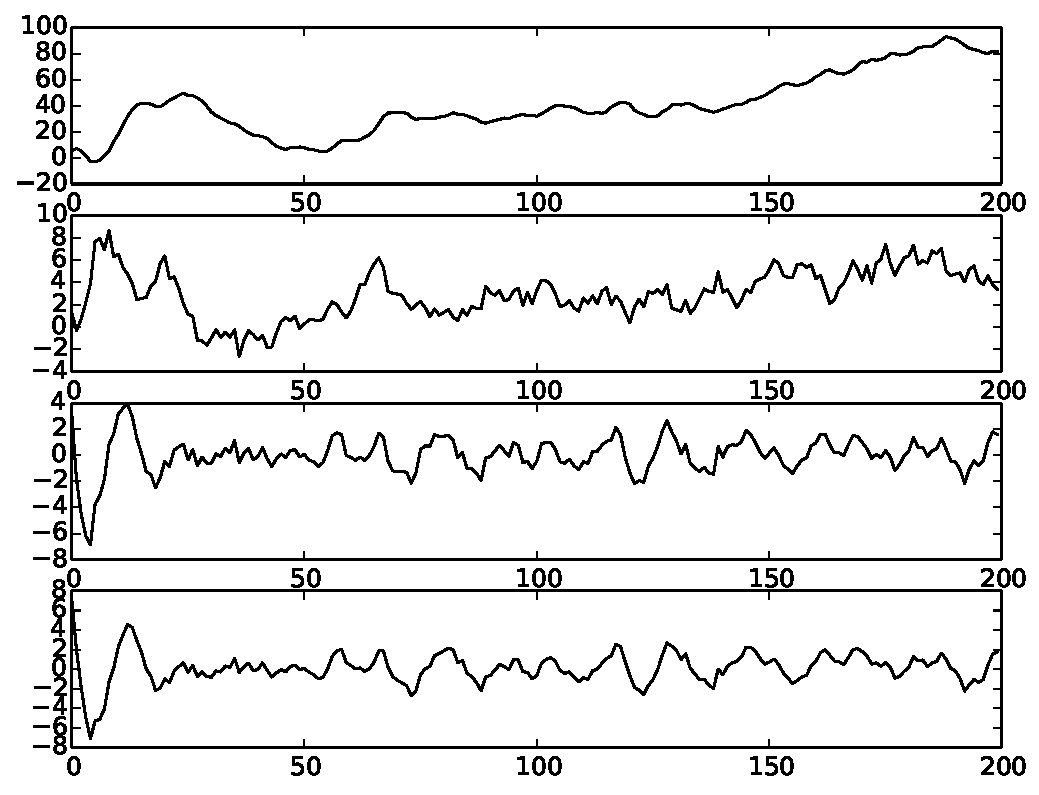
\includegraphics[width=0.9\columnwidth]{figures/toy-state.pdf}
 \caption{An example data set simulated from the toy model, showing evolution of the four state components over time.}
 \label{fig:toy-data}
\end{figure}

\begin{figure}
 \centering
 \subfloat[]{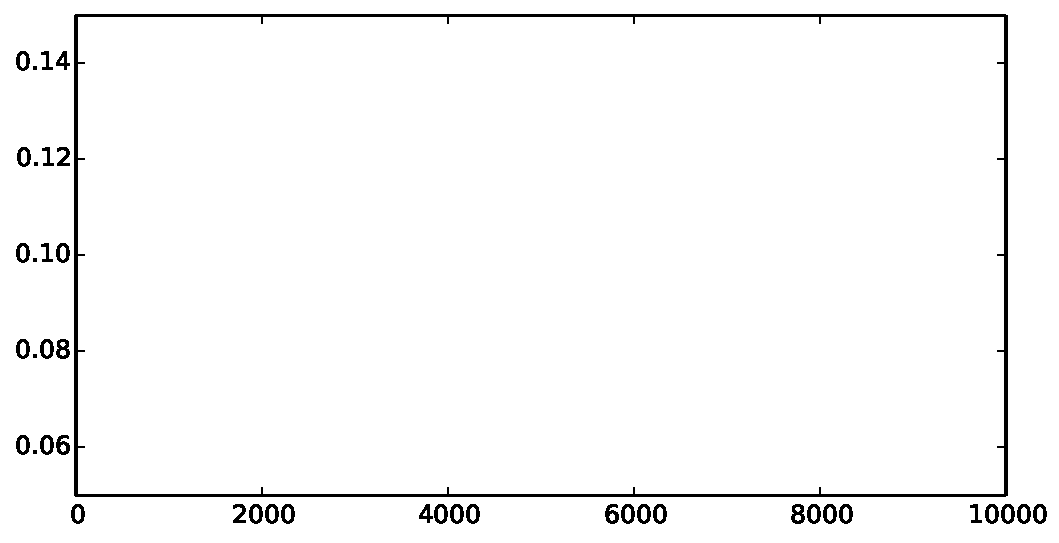
\includegraphics[width=0.9\columnwidth]{figures/toy-basic-R-trace.pdf} \label{subf:toy-R-trace:basic}} \\
 \subfloat[]{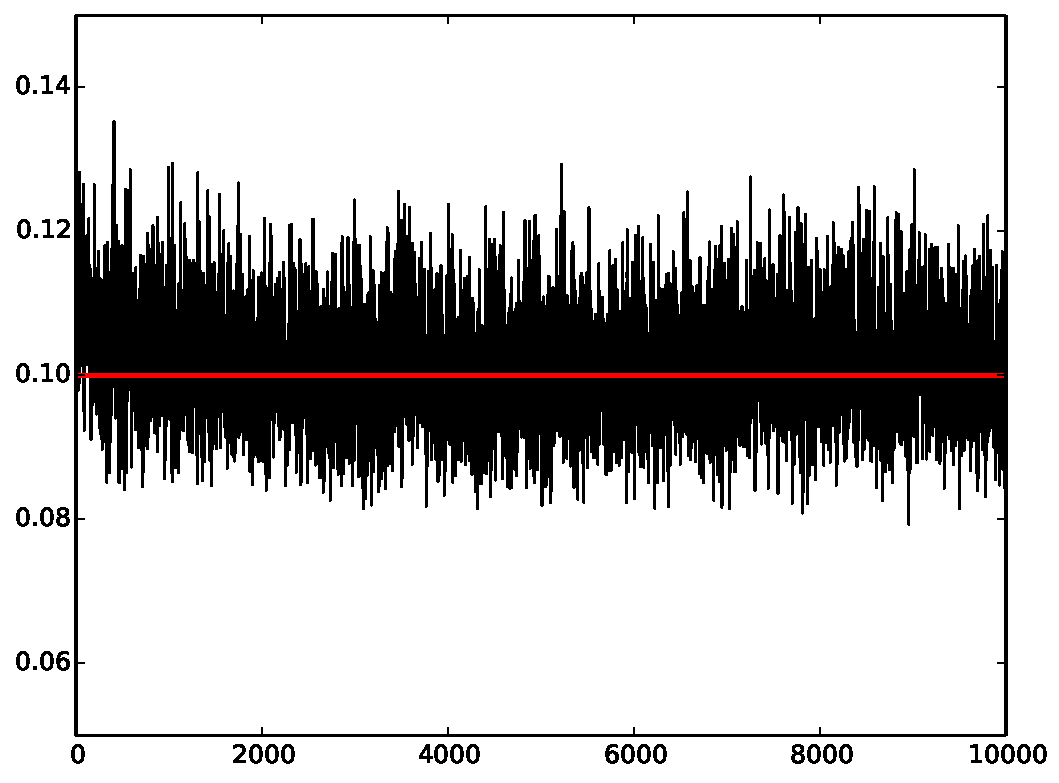
\includegraphics[width=0.9\columnwidth]{figures/toy-degenerate-R-trace.pdf} \label{subf:toy-R-trace:degenerate}}
 \caption{MCMC trace plots for $\xi_{\ob{}}$ for the full rank transition model \protect\subref{subf:toy-R-trace:basic} and the degenerate transition model \protect\subref{subf:toy-R-trace:degenerate}.}
 \label{fig:toy-R-trace}
\end{figure}

\begin{figure}
 \centering
 \subfloat[]{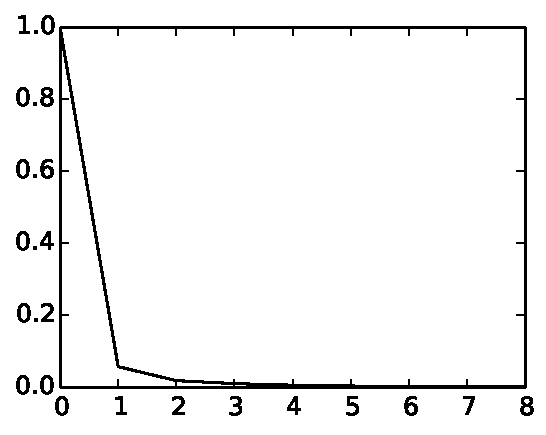
\includegraphics[width=0.45\columnwidth]{figures/toy-basic-R-acf.pdf} \label{subf:toy-R-acf:basic}}
 \subfloat[]{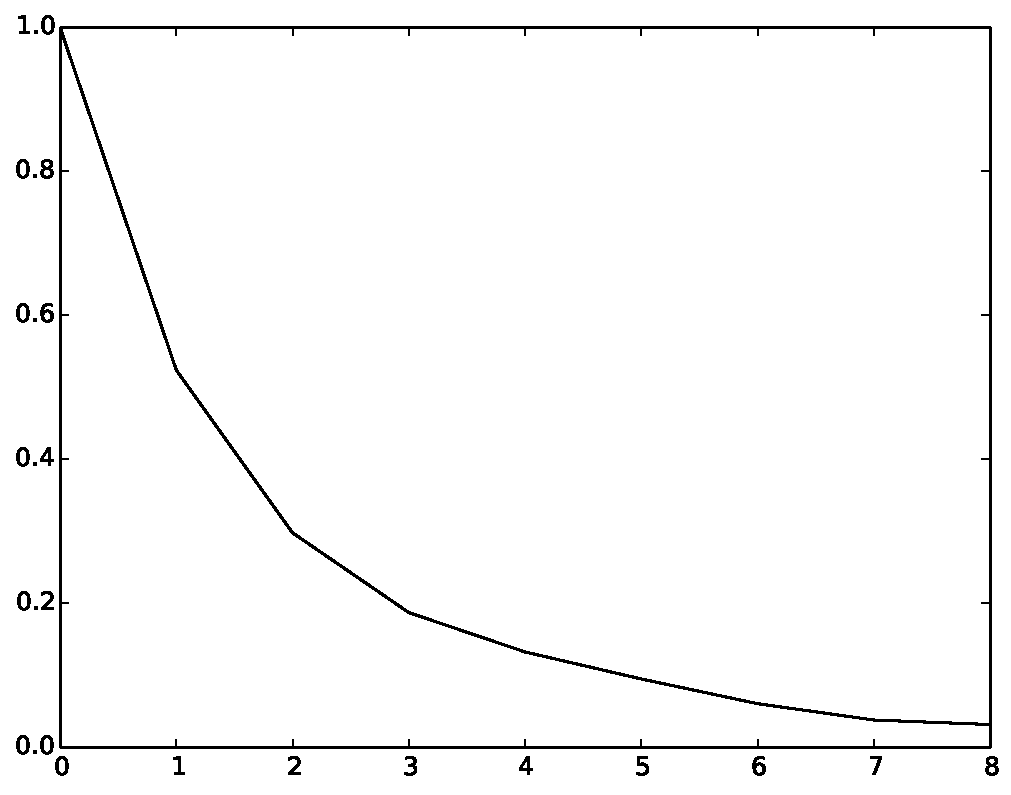
\includegraphics[width=0.45\columnwidth]{figures/toy-degenerate-R-acf.pdf} \label{subf:toy-R-acf:degenerate}}
 \caption{MCMC autocorrelation plots for $\xi_{\ob{}}$ for the full rank transition model \protect\subref{subf:toy-R-acf:basic} and the degenerate transition model \protect\subref{subf:toy-R-acf:degenerate}.}
 \label{fig:toy-R-acf}
\end{figure}

\begin{figure}
 \centering
 \subfloat[]{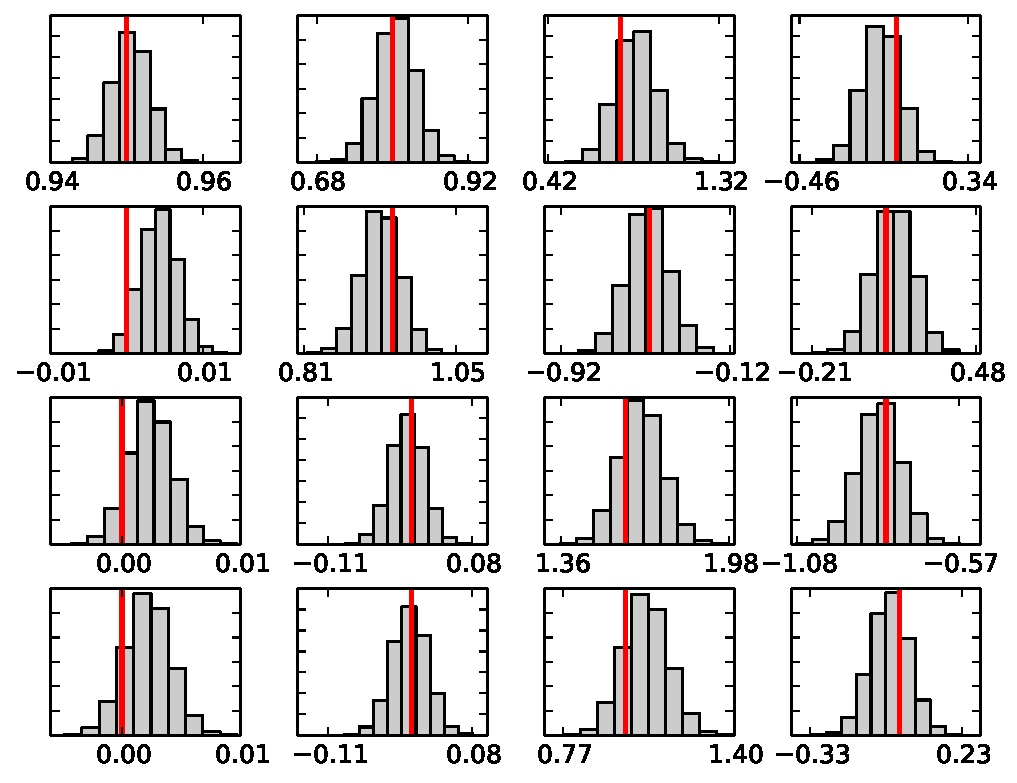
\includegraphics[width=0.9\columnwidth]{figures/toy-degenerate-F-hist.pdf} \label{subf:toy-FQ-hist:F}} \\
 \subfloat[]{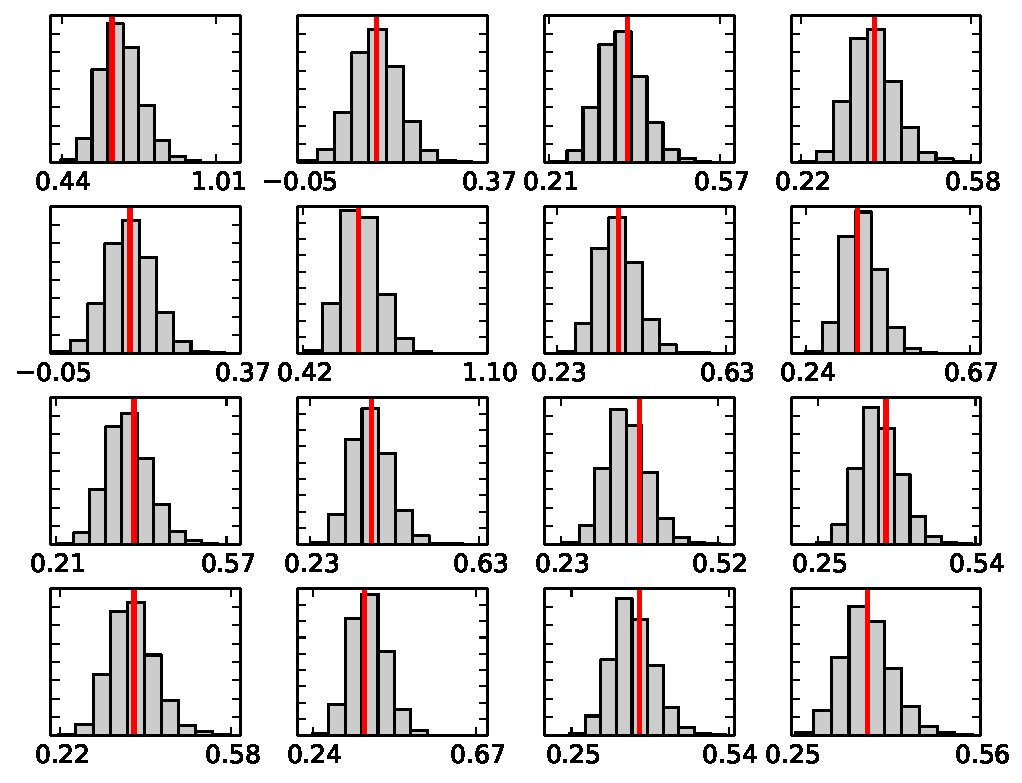
\includegraphics[width=0.9\columnwidth]{figures/toy-degenerate-Q-hist.pdf} \label{subf:toy-FQ-hist:Q}}
 \caption{MCMC Posterior histograms for \protect\subref{subf:toy-FQ-hist:F} $\lgtm$ and \protect\subref{subf:toy-FQ-hist:Q} $\lgtv$, from the degenerate linear transition model. Vertical lines indicate true values}
 \label{fig:toy-FQ-hist}
\end{figure}



\subsection{Motion Capture Interpolation} \label{sec:mocap}

In a more realistic example, the MCMC algorithms are applied to the problem of marker interpolation in a motion capture application. The data used is from \cite{Aristidou2013}. A motion capture system was used to measure the $3$-dimensional coordinates of a number of markers attached to a subject's body. Here we consider the four markers attached to the head. Since these are all attached to the same rigid body, we expect there to be substantial correlation in their motion. Sometimes markers are occluded meaning that position measurements are missing. If a system model for the motion of the markers can be learned, then the missing marker locations can be inferred by sampling or Kalman smoothing.

The original data is down-sampled to $5$Hz, and consists of $250$ time instants with occasional measurements missing due to occlusion. Observations from one marker at a time are discarded in $4$ sections each of $20$ time instants (i.e. $4$s each). The remaining observations are used to learn various system models with MCMC, and performance is assessed by comparing the root-mean-square error (RMSE) of the inferred positions in the missing sections. The data set is shown in figure~\ref{fig:mocap_data}.

\begin{figure}
 \centering
 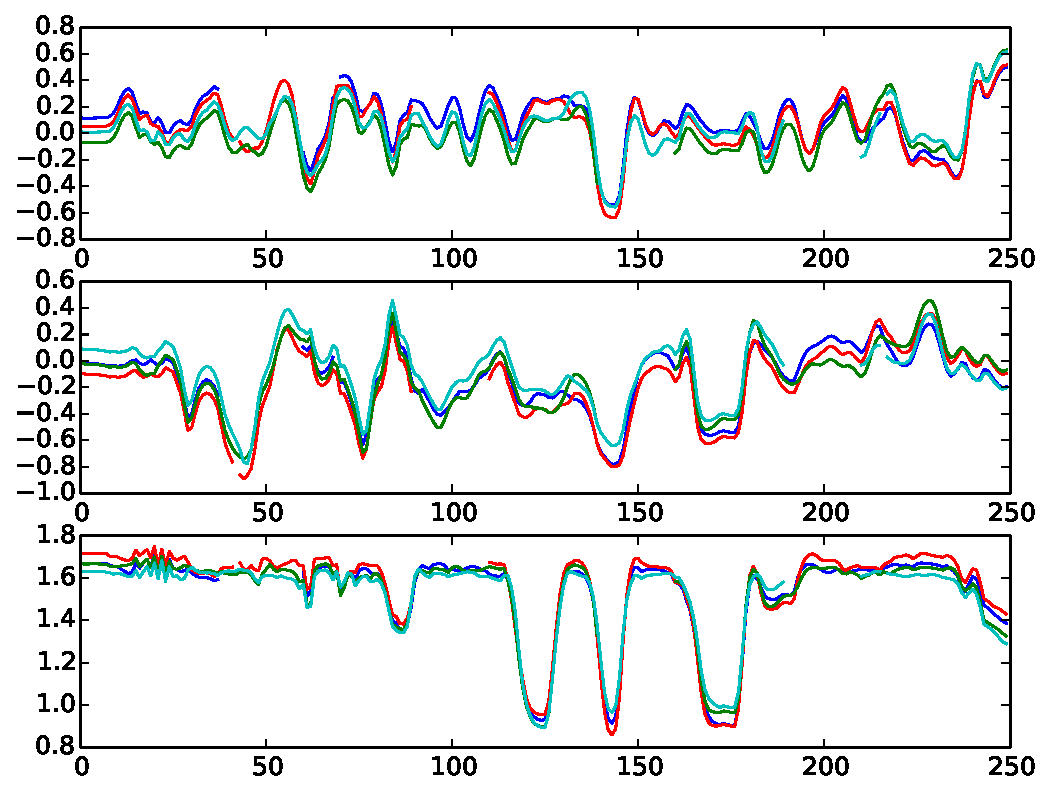
\includegraphics[width=0.9\columnwidth]{figures/mocap-data.pdf}
 \caption{Motion capture data. Showing the three position coordinates over time for each of the four head markers.}
 \label{fig:mocap_data}
\end{figure}

We assume that the latent state consists of $3$-dimensional position and velocity for each marker in Cartesian coordinates,
%
\begin{IEEEeqnarray}{rCl}
 \ls{\ti} & = & \begin{bmatrix}
                 \mathbf{r}_{\ti} \\ \mathbf{v}_{\ti}
                \end{bmatrix} \nonumber     .
\end{IEEEeqnarray}
%
The observation model is defined by the following matrices,
%
\begin{IEEEeqnarray}{rCl}
 \lgom &=& \begin{bmatrix} \idmat & \zmat \end{bmatrix} \\
 \lgov &=& \xi_{\ob{}} \idmat     .
\end{IEEEeqnarray}

Three transition models are trained using MCMC:
%
\begin{itemize}
 \item A near constant velocity motion (NCVM) model \cite{Li2003} in which the motion of each marker is assumed independent from the rest.
 \item A standard linear model, with full rank $\lgtv$.
 \item A degenerate linear model, with $\lgtv$ singular and of unknown rank.
\end{itemize}
%
The near constant velocity model has the following system matrices,
%
\begin{IEEEeqnarray}{rCl}
 \lgtm &=& \begin{bmatrix}
            \idmat & \idmat \\ \zmat & \idmat
           \end{bmatrix} \\
 \lgtv &=& \xi_{\ls{}} \begin{bmatrix}
            \frac{1}{3}\idmat & \half\idmat \\ \half\idmat & \idmat
           \end{bmatrix}     .
\end{IEEEeqnarray}
%
$\xi_{\ls{}}$ is an unknown which may be learned within the MCMC scheme using Gibbs moves.

The hyperparameters are set to the same uninformative values as for the toy model, with the following exception,
%
\begin{IEEEeqnarray}{rCl}
 \priorscalematrix &=& 0.001 \priordof \idmat \nonumber \\
 \priorscalematrixbase &=& 0.001 \idmat \nonumber \\
 \priortypval &=& 0.01     .
\end{IEEEeqnarray}

Each MCMC algorithm is run for $20000$ iterations, of which the first $10000$ are discarded as burn-in. The sampler for the degenerate model displays very similar behaviour as with the toy model. In the first few hundred iterations the parameters alter rapidly, and the covariance rank is reduced to a value of $9$, where it remains thereafter. The Metropolis-Hastings moves continue to alter the system matrices until the chain appears to converge after about $5000$ iterations.

For each model, an estimate of the position of the missing markers is made by taking the mean of the sampled state trajectories from the Markov chain. The resulting RMSE is then calculated. For comparison, a missing value singular value decomposition (MSVD) algorithm is also tested \cite{Srebro2003,Liu2006,Li2009}, in which we use components sufficient to capture $95\%$ of the energy in each iteration. The RMSE results are shown in table~\ref{tab:mocap-rmse}.

\begin{table}
 \centering
 \begin{tabular}{l|l}
  Model          & RMSE \\
  \hline
  NCVM           & 4.692 \\
  Basic          & 0.154 \\
  Degenerate     & 0.086 \\
  MSVD           & 0.926
 \end{tabular}
 \caption{Root-mean-square error (RMSE) for estimated missing marker positions, in metres.}
 \label{tab:mocap-rmse}
\end{table}



\section{Discussion and Conclusions}

Markov chain Monte Carlo algorithms are an effective method for Bayesian learning of linear state space systems. In this paper, we have introduced new MCMC kernels for learning linear state space models which may have a singular transition covariance matrix of unknown rank. Such degenerate models may provide a better mathematical description of some systems, when the number of independent components in the state transitions is lower than the number of state dimensions. When a degenerate model is appropriate, the state estimates it produces can be more accurate than those obtained from an equivalent full rank model, as we have shown in simulations. Furthermore, with the rank of the transition covariance matrix included in the model, the sampler provides an explicit estimate of the posterior distribution over this parameter.

The price for using a degenerate transition model is an increased computational cost of the MCMC simulation. The computational complexity is the same as the full rank algorithm, dominated by the Kalman filtering and backward sampling operations which are $\bigo{\lsd^3 \timax}$. However, the need for additional Metropolis-Hastings steps increases the cost per iteration. More significantly, the Markov chain mixes more slowly and thus requires a longer chain to be simulated to achieve the same effective sample size. An important avenue for future research will be designing more sophisticated Metropolis-Hastings moves to explore the parameters space more efficiently than the simple random walks used here.

The standard linear Gaussian state space models, with $\rank(\lgtv)=\lsd$, discussed in section~\ref{sec:linear_gaussian_models} are a special case of the more general class used thereafter, for which $\rank(\lgtv)$ was treated as unknown. Correspondingly, the MCMC algorithm for the general case reduces to the standard Gibbs sampler of section~\ref{sec:linear_gaussian_models} if we re-impose the constraint that $\rank(\lgtv)=\lsd$. In this case $\tvfull=\lgtv$, $\tvrot=\idmat$, the ``constrained'' Gibbs moves are no longer constrained, and the Metropolis-Hastings moves become redundant.



\section*{Acknowledgements}
The authors are supported by the EPSRC BTaRoT grant. Our thanks to Michael Burke for advice and assistance with the motion capture application, and to Rich Wareham for his geometric insights.


\appendices

\section{A~Matrix~Factorisation for Positive~Semi-Definite~Matrices} \label{app:givens-factorisation}

A Givens rotation matrix has the following structure,
%
\begin{IEEEeqnarray}{rCl}
 \left[\givmat{i}{j}{\givrot{}} - \idmat\right]_{k,l} & = & \begin{cases}
                                                    \cos(\givrot{})-1 & k=l=i \text{ or } k=l=j \\
                                                    \sin(\givrot{}) & k=i,l=j \\
                                                    -\sin(\givrot{}) & k=j,l=i \\
                                                    0 & \text{ otherwise}     ,
                                                 \end{cases}
\end{IEEEeqnarray}
%
where $\givrot{} \in [-\pi/2,\pi/2]$ is a rotation in the plane of the $i$ and $j$ coordinate directions. Any orthogonal $d\times d$ matrix may be written as a product of $\half d(d-1)$ such rotations in the following way \cite{Anderson1987},
%
\begin{IEEEeqnarray}{rCl}
\tvvec = \tvsign &\times& \left[ \givmat{1}{2}{\givrot{1,2}}\right] \times \dotsm \nonumber\\
&\times& \left[\givmat{1}{d-1}{\givrot{1,d-1}} \dotsm \givmat{d-2}{d-1}{\givrot{d-2,d-1}} \right] \nonumber\\
&\times& \left[\givmat{1}{d}{\givrot{1,d}} \dotsm \givmat{d-1}{d}{\givrot{d-1,d}} \right] \label{eq:standard_givens}     ,
\end{IEEEeqnarray}
%
where $\tvsign$ is a diagonal matrix in which the diagonal elements are $\pm1$. This factorisation may be derived (and also calculated) by iteratively left multiplying the original matrix by a Givens rotation matrix such that one element is set to $0$. The matrix remaining once all the elements below the diagonal have been eliminated is $\tvsign$, and the factorisation above results from a straightforward rearrangement. See \cite{Anderson1987} for details. This factorisation is not unique. Any order of Givens matrices may be used provided each operation does not interfere with the elements zeroed by the preceding operations. Furthermore, we can also zero an element of the matrix by right multiplication by a Givens matrix, so the rotations may be split into two blocks, one each side of the sign matrix.

Now consider instead a $d \times r$ matrix of orthogonal columns. This can be factorised using the same mechanism. First right multiply by Givens matrices to zero the elements on the first $r$ rows below the main diagonal. Then left multiply by Givens matrices to zero all the elements on rows $r+1$ to $d$. The resulting factorisation is,
%

\begin{IEEEeqnarray}{rCl}
 \tvvec & = & \tvcross \tvsign \tvrow      ,
\end{IEEEeqnarray}
%
where
%
\begin{IEEEeqnarray}{rCl}
 \tvrow  & = & \left[\givmat{1}{2}{\givrot{1,2}}\right] \times \dotsm \nonumber \\
 & & \qquad\qquad \times \left[\givmat{1}{r}{\givrot{1,r}} \dots \givmat{r-1}{r}{\givrot{r-1,r}}\right] \\
 \tvcross & = & \left[\givmat{1}{r+1}{\givrot{1,r+1}}\dots\givmat{1}{d}{\givrot{1,d}}\right] \times \dotsm \nonumber \\
 & & \qquad\qquad \times \left[\givmat{r}{r+1}{\givrot{r,r+1}} \dots \givmat{r}{d}{\givrot{r,d}}\right]      ,
\end{IEEEeqnarray}
%
and $\tvsign$ is as before, with the following structure,
%
\begin{IEEEeqnarray}{rCl}
 \tvsign & = & \begin{bmatrix}
                  \tvsigndiag \\
                  \zmat[(d-r)\times r]
                 \end{bmatrix} \nonumber      .
\end{IEEEeqnarray}

Now consider a rank-$r$ positive semi-definite matrix $\psd$ for which the non-singular part of the eigendecomposition is,
%
\begin{IEEEeqnarray}{rCl}
 \psd &=& \tvvec \tvval \tvvec\tr     . 
\end{IEEEeqnarray}
%
Factorising the matrix of eigenvectors using the Givens method, we find,



\begin{IEEEeqnarray}{rCl}
 \psd & = & \tvcross \tvsign \tvrow \tvval \tvrow\tr \tvsign\tr \tvcross\tr  \nonumber \\
 & = & \tvcross \begin{bmatrix}
                  \tvsigndiag \tvrow \tvval \tvrow\tr \tvsigndiag\tr & \zmat \\
                  \zmat & \zmat
                \end{bmatrix} \tvcross\tr \nonumber \\
 & = & \tvrot \tvfull \tvrot\tr \nonumber      ,
\end{IEEEeqnarray}
%
in which $\tvrot$ consists of the first $r$ columns of $\tvcross$, and,
%
\begin{IEEEeqnarray}{rCl}
 \tvfull &=& \tvsigndiag \tvrow \tvval \tvrow\tr \tvsigndiag\tr    .
\end{IEEEeqnarray}
%
Comparing with \eqref{eq:standard_givens}, we see that $\tvsigndiag \tvrow$ is an unconstrained $r\times r$ orthogonal matrix and hence $\tvfull$ is a unique positive definite matrix.


\bibliographystyle{IEEEtran}
\bibliography{/home/pete/Dropbox/PhD/bibliographies/Cleanbib}
% \bibliography{/home/pete/Dropbox/PhD/bibliographies/OTbib}
\end{document}



\end{document}
